\chapter{Introduction}
\graphicspath{{Chapter1/Figs/}{Chapter1/Figs/}}

This chapter introduces the reader to the primary focus of this thesis and introduces key topics and their explanations. It also displays the research question, aims, objectives, and distinctions of the thesis's primary contents and structure.

\section{Background}
\label{chapter1-background}

There has been a long-standing interest in developing neural interfaces, systems that sense electrical impulses from the nervous system and use them to intercommunicate with the human brain. Successful research into the development of technologies that enable neural interfaces has been going on for decades, with the first experiments being conducted by Jacques J. Vidal in the late 1970s \citep{vidal_real-time_1977}. Progress has accelerated significantly in the past few years, especially since the advent of modern processing capabilities such as in deep learning with convolutional neural networks (CNN) or generative adversarial networks (GAN) \citep{gonfalonieri_deep_2019}. In particular, a related discipline called brain-computer interfacing (BCI), a field focused on the direct interaction between brains and computers, has accumulated much momentum since the popularity of companies like Neuralink and Kernel.

One aspect of neural interfaces is hardware tailored to the human body. Whether it is an invasive sensor, such as in electrocorticography (ECoG), a method which uses electrodes placed on the surface of the brain, or a non-invasively placed sensor on the body, such as in electroencephalography (EEG). Both methods measure electrical activities produced by neurons; however, with decreasing spatial precision, the farther the electrode is placed from the brain, the more body structures (e.g. bones) are between firing neurons and the measuring sensor. The other aspect is software that reads and interprets data of these hardware sensors. Both aspects present their own set of challenges and complexities. Nonetheless, complete and applicable neural interfaces work in practice and have been used for many years in patients with neurological disorders \citep{braingate_publications_nodate}. There are also consumer and non-clinical neural interfaces available, such as the Neurosity and OpenBCI products, which aim to democratise the use of EEG sensors by offering low-cost hardware and simple-to-use software.

\section{Relevance}
\label{chapter1-relevance}

\begin{figure}
  \centering
  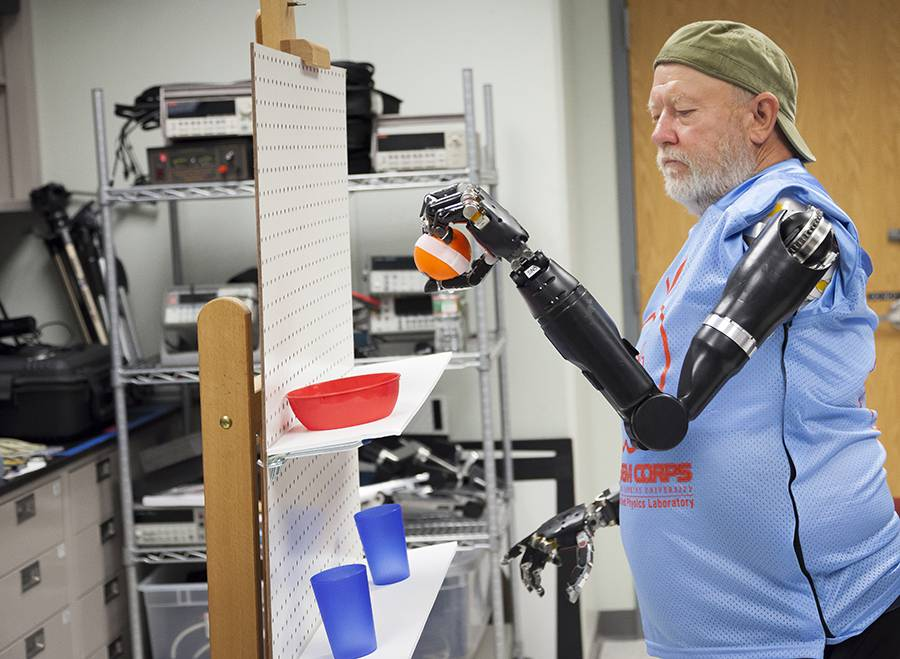
\includegraphics[width=\linewidth]{prostetic-arms.jpg}
  \caption{Les Baugh, an amputee, is using a neural interface to control two robotic arms with his thoughts \citep{campbell_amputee_2014}.}
  \label{fig:prostetic-arms}
\end{figure}

The possibilities of connecting the human brain with computers are almost limitless because one has to think that we are the brain, that our own perception of reality, all our feelings, memories and actions are supposed to be contained in the electrical impulses of our brain. The ability to communicate directly with our thoughts and the outside world — whether through digital or physical objects — is a fantastic prospect. There are several use cases: Controlling prosthetic limbs for amputees \citep{murphy_electroencephalogram-based_2017}, communication for people with locked-in syndrome \citep{chaudhary_spelling_2022}, diagnosing neurological problems and improving the mental capacities of elderly patients \citep{belkacem_brain_2020} are promising examples, to name a few.

It may appear evident that neural interfaces can significantly impact the field of therapeutics and accessibility for a small subset of the human population. However, one can envision not only alleviating deplorable living conditions but also improving the lives of healthy people through more natural or efficient ways of interacting with things or by directly altering human brains for certain benefits. Because most current neural interface applications concentrate on the first aspect of therapeutics and accessibility, other use cases, such as stimulating the brain to improve concentration, modifying cognitive load, or even uploading new knowledge directly into the brain, may appear to be science fiction ideas.

Regardless, many capable people — research labs and even entire companies — are developing neural interface hardware and software aimed at the general population without conditions that envision a future for such use cases in the long term. The applicability of a neural interface system to the mainstream will depend on several factors, presumably an important factor of which is the hardware's form factor. Nonetheless, the totality of the ecosystem in which the software resides is a valuable aspect that should not be overlooked.

\section{Research question}
\label{chapter1-research-question}

\begin{figure}[ht]
  \centering
  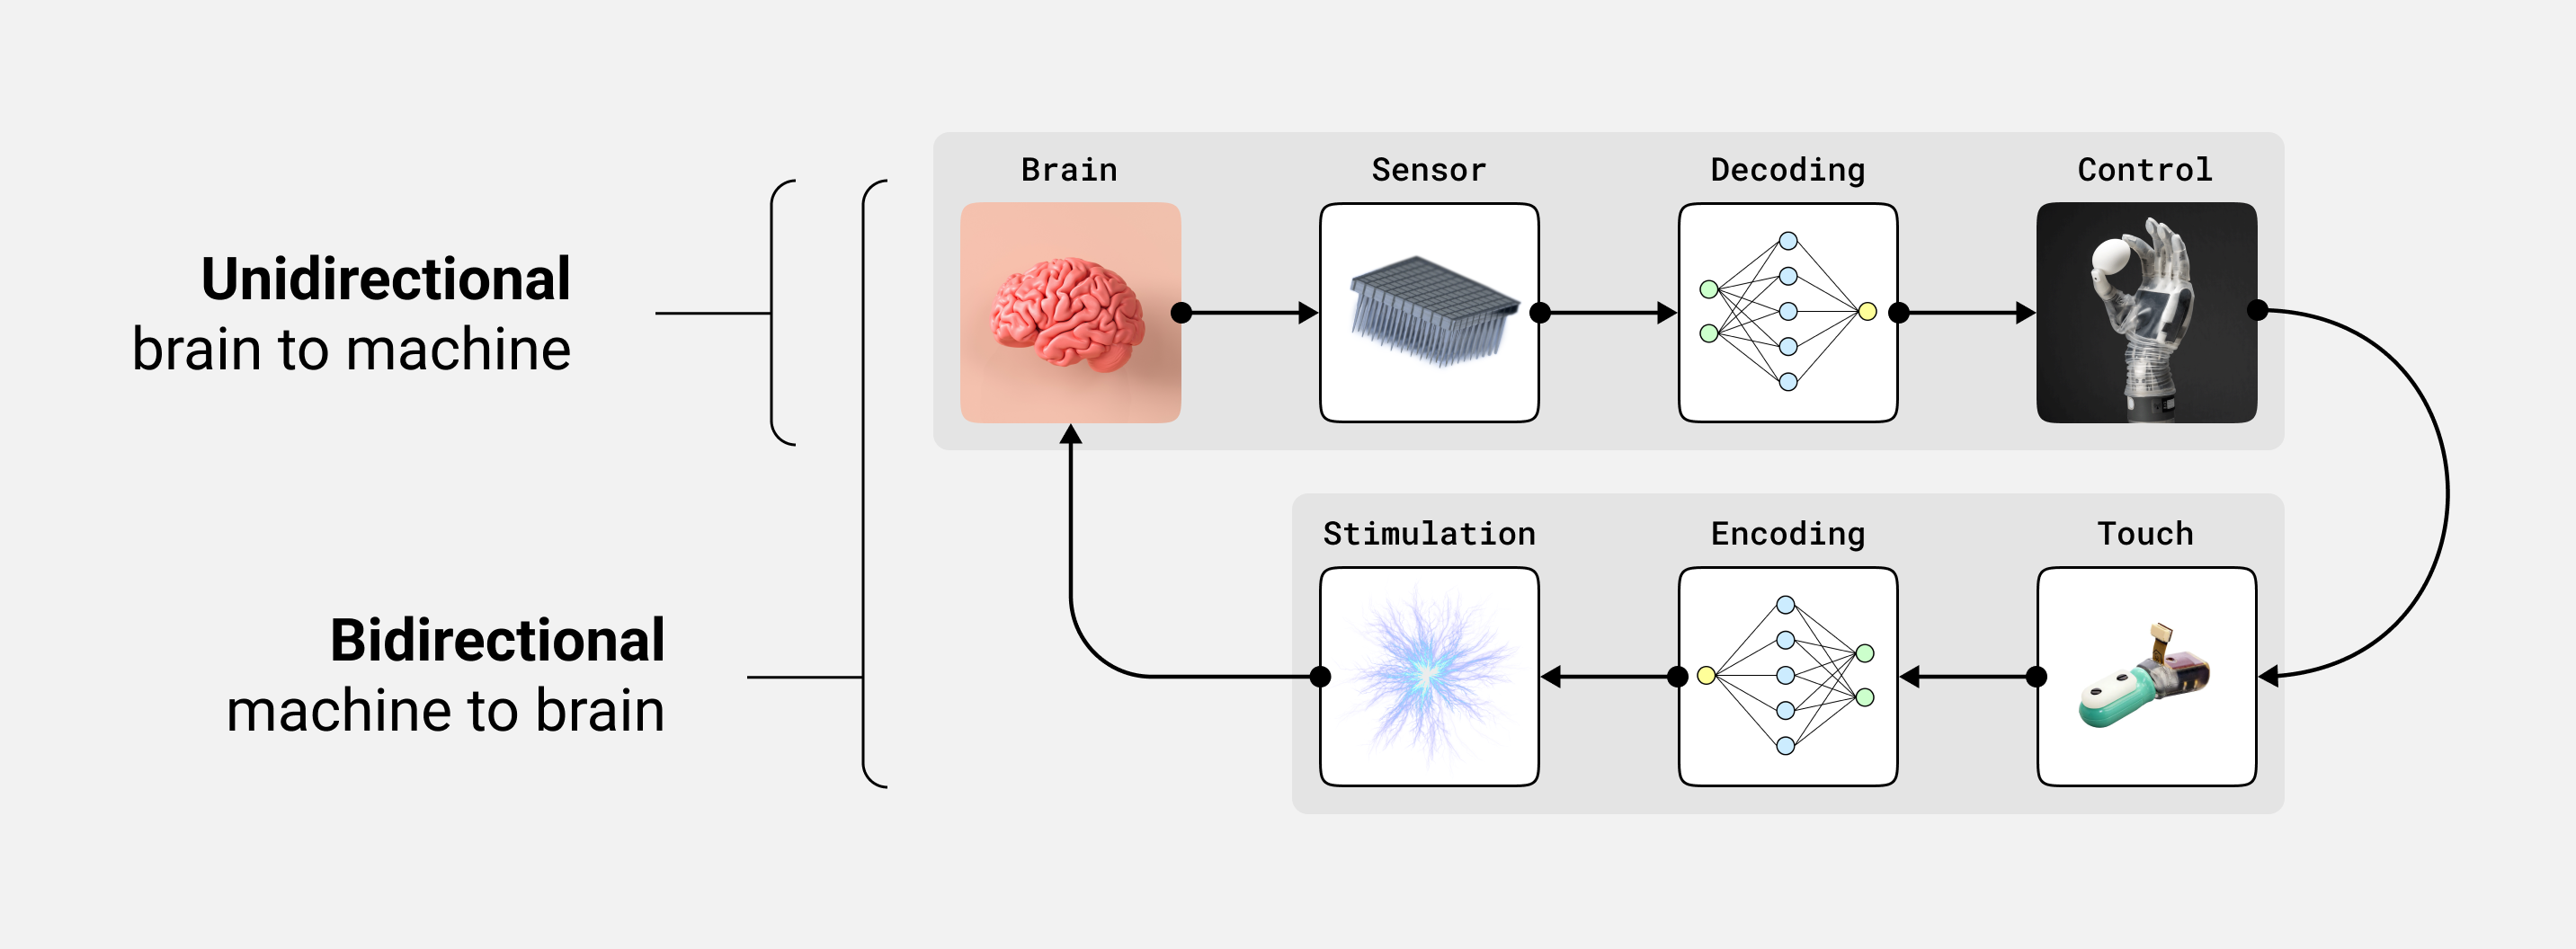
\includegraphics[width=\linewidth]{directional-system.png}
  \caption{Difference between an unidirectional and bidirectional neural interface and its components (own representation, 2022).}
  \label{fig:directional-system}
\end{figure}

Whether it is a bidirectional and invasive neural interface with the potential to be implanted on a large scale, as e.g. Neuralink is aiming to do, or a unidirectional and non-invasive interface in various form factors that are also aimed at the mass market, such as in a pair of glasses or a pair of headphones, the data collected from the brain would always need to be processed, contextualised, and classified to produce an intelligible output. The research question of the present thesis is on determining what technical components such a software system would require to be production-ready and suitable for a mass-market product. The emphasis is on a holistic view of such a system, which means that the entire technology stack is taken into account in answering the research question.

Furthermore, most current neural interface software systems in production, for example, for an interface implanted in a living patient, are typically run in a local environment, i.e. the software system and its components are typically located on a physically nearby computer, usually connected by a cable, to reduce latency and avoid complexities introduced by a wireless protocol. There is already promising research on wireless mobile brain-computer interfaces (mBCI) by \citeauthor{minguillon_mobile_2017} \citeyearpar{minguillon_mobile_2017} or possible implications of human brain/cloud interfaces (B/CI) by \citeauthor{martins_human_2019} \citeyearpar{martins_human_2019} or by \citeauthor{angelica_cognitive_2021} \citeyearpar{angelica_cognitive_2021}, which analyse bringing hypothetical future large-scale brain-computer interface software systems into the cloud.

\nomenclature[mbci]{mBCI}{Mobile brain-computer interface}
\nomenclature[bc-i]{B/CI}{Brain/cloud interface}

\section{Hypothesis}
\label{chapter1-hypothesis}

Previous research on brain/cloud interfaces has tended to focus on speculations based on hypothetical scenarios in the future, usually based on the premise of other developed technologies such as neural nanorobotics, vital advances in 5G, or the presence of supercomputers in the cloud, e.g. for the augmentation of the human brain, or a communication network for brain-to-brain interfacing (BTBI), and are thus rather distant from today's pertinence. To distinguish the research presented in this thesis, the author coins the term neural/cloud interface (N/CI), which refers to a holistic software interface that connects a neural interface device to the cloud and then to other neural interfaces, software applications, cloud systems, or physical devices.

The primary hypothesis is that a neural/cloud interface is feasible with modern software technologies, requiring only theoretical groundwork based on empirical engineering in a deployable and producible system. This thesis looks at the process and lessons learned from the author's perspective developing a N/CI in the industry for an actual mainstream-capable neural interface device for a BCI end-user application to shed more light on this.

\section{Goals and aims}
\label{chapter1-goals-and-aims}

The overall goal of this thesis is to give the reader an overview of the definition of a N/CI, its components, and the lessons learned in building a reproducible production-grade, and end-user facing N/CI application with a non-invasive, unidirectional neural interface hardware. In addition to the overall goal, the thesis aims to illustrate a powerful demonstration of the possibilities of neural interfaces on the World Wide Web for virtual reality (VR) or augmented reality (AR) applications running in a browser environment in order to exemplify how to extend the human-computer interaction (HCI) for future 3D applications when combined with a BCI.

\section{Objectives}
\label{chapter1-objectives}

The hypothesis of the present thesis states that an N/CI is realisable with contemporary technologies and thus distinguishes itself from previous work with the term brain/cloud interface from \citeauthor{martins_human_2019}, which, as already mentioned, rather aims at speculative future scenarios. Based on the research question of which components make up an N/CI, the goal is to establish a holistic N/CI and thus identify and evaluate suitable methods for creating such an N/CI. In order to achieve this goal, the author must achieve the following objectives:

\begin{enumerate}
  \item Identify and illustrate the most relevant software components required to realise a production-grade N/CI.
  \item Identify and deploy the most effective software components in a given and appropriate context to build a production-grade N/CI.
  \item Develop and publicly release an example N/CI application codebase that is easy to understand and extend.
  \item Demonstrate the applicability and impact for HCI of a N/CI with web-based VR/AR applications.
\end{enumerate}

\nomenclature[cnn]{CNN}{Convolutional neural networks}
\nomenclature[gan]{GAN}{Generative adversarial networks}
\nomenclature[bci]{BCI}{Brain-computer interface}
\nomenclature[ecog]{ECoG}{Electrocorticography}
\nomenclature[eeg]{EEG}{Electroencephalography}
\nomenclature[btbi]{BTBI}{Brain-to-brain interfaces}
\nomenclature[nci]{N/CI}{Neural/cloud interface}
\nomenclature[vr]{VR}{Virtual reality}
\nomenclature[ar]{AR}{Augmented reality}
\nomenclature[hci]{HCI}{Human-computer interaction}
